\documentclass[12pt]{article}
\usepackage[T1, T2A]{fontenc}
\usepackage[utf8]{inputenc}
\usepackage[russian]{babel}
\usepackage{hyperref}
\usepackage{graphicx}
\graphicspath{ {../Images/} }

\author{Григорий Матюхин}
\date{\today}
\title{Лабораторная работа \textnumero10.\\Основы работы с модулями ядра операционной системы}

\begin{document}
\maketitle
\newpage
\tableofcontents
\newpage
\section{Цель работы}
Получить навыки работы с утилитами управления модулями ядра операционной системы.

\section{Последовательность выполнения работы}
\subsection{Управление модулями ядра из командной строки}
\begin{enumerate}
	\item Запустите терминал и получите полномочия администратора:
	\item Посмотрите, какие устройства имеются в вашей системе и какие модули ядра с ними связаны:
	      \\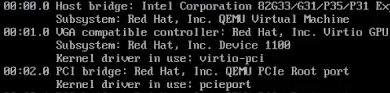
\includegraphics{1.png}
	\item Посмотрите, какие модули ядра загружены:
	      \\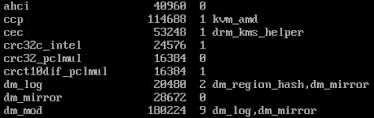
\includegraphics{2.png}
	\item Посмотрите, загружен ли модуль \texttt{ext4}:
	      \\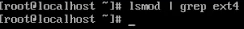
\includegraphics{3.png}
	\item Загрузите модуль ядра \texttt{ext4}. Убедитесь, что модуль загружен, посмотрев список загруженных модулей:
	      \\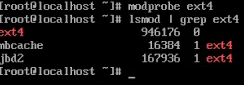
\includegraphics{4.png}
	\item Посмотрите информацию о модуле ядра \texttt{ext4}:
	      \\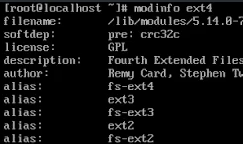
\includegraphics{5.png}
	\item Попробуйте выгрузить модуль ядра \texttt{ext4}:
	      \\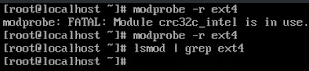
\includegraphics{6.png}
	\item Попробуйте выгрузить модуль ядра \texttt{xfs}:
	      \\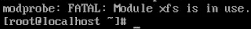
\includegraphics{7.png}
\end{enumerate}

\subsection{Загрузка модулей ядра с параметрами}
\begin{enumerate}
	\item Запустите терминал и получите полномочия администратора.
	\item Посмотрите, загружен ли модуль \texttt{bluetooth}:
	\item Загрузите модуль ядра \texttt{bluetooth}:
	      \\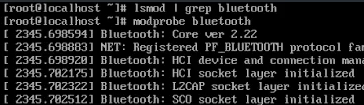
\includegraphics{8.png}
	\item Посмотрите список модулей ядра, отвечающих за работу с \texttt{bluetooth}:
	      \\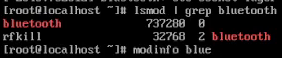
\includegraphics{9.png}
	\item Посмотрите информацию о модуле \texttt{bluetooth}:
	      \\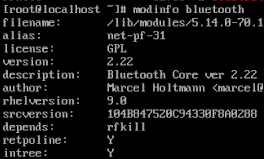
\includegraphics{10.png}
	\item Выгрузите модуль ядра \texttt{bluetooth}:
	      \\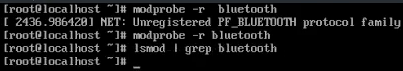
\includegraphics{11.png}
\end{enumerate}

\subsection{Обновление ядра системы}
\begin{enumerate}
	\item Запустите терминал и получите полномочия администратора:
	\item Посмотрите версию ядра, используемую в операционной системе:
	      \\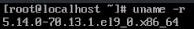
\includegraphics{12.png}
	\item Выведите на экран список пакетов, относящихся к ядру операционной системы:
	      \\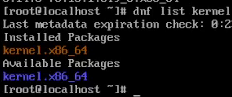
\includegraphics{13.png}
	\item Обновите систему, чтобы убедиться, что все существующие пакеты обновлены, так как это важно при установке/обновлении ядер \texttt{Linux} и избежания конфликтов:
	      \\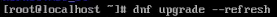
\includegraphics{14.png}
	\item Обновите ядро операционной системы, а затем саму операционную систему:
	      \\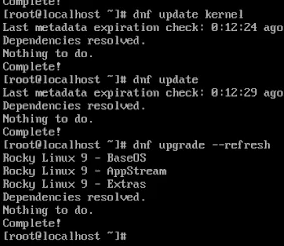
\includegraphics{15.png}
	\item Перегрузите систему. При загрузке выберите новое ядро.
	      \\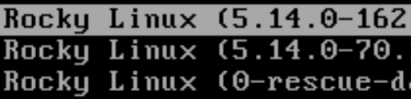
\includegraphics{16.png}
	\item Посмотрите версию ядра, используемую в операционной системы:
	      \\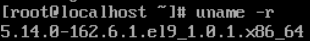
\includegraphics{17.png}
\end{enumerate}

\section{Контрольные вопросы}
\begin{enumerate}
	\item Какая команда показывает текущую версию ядра, которая используется на вашей системе? \\
	      \texttt{uname -r}
	\item Как можно посмотреть более подробную информацию о текущей версии ядра операционной системы? \\
	      \texttt{hostnamectl}
	\item Какая команда показывает список загруженных модулей ядра? \\
	      \texttt{lsmod}
	\item Какая команда позволяет вам определять параметры модуля ядра? \\
	      \texttt{modinfo <mod-name>}
	\item Как выгрузить модуль ядра? \\
	      \texttt{modprobe -r <mod-name>}
	\item Что вы можете сделать, если получите сообщение об ошибке при попытке выгрузить модуль ядра? \\
	      Завершить все процессы, использующие модуль и повторить снова.
	\item Как определить, какие параметры модуля ядра поддерживаются? \\
	      Ввести команду \texttt{modinfo <mod-name>} и посмотреть на \texttt{parm} строки.
	\item Как установить новую версию ядра? \\
	      \begin{enumerate}
		      \item Обновить существующие пакеты: \texttt{dnf upgrade --refresh}
		      \item Обновить ядро операционной системы: \texttt{dnf update kernel}
		      \item Обновить операционную систему: \texttt{dnf update}
	      \end{enumerate}
\end{enumerate}

\section{Вывод}
В ходе выполнения данной работы я получил навыки работы с утилитами управления модулями ядра операционной системы.

\end{document}
